%%%%%%%%%%%%%%%%%%%%%%%%%%%%%%%%%%%%%%%%%
% baposter Landscape Poster
% LaTeX Template
% Version 1.0 (11/06/13)
%
% baposter Class Created by:
% Brian Amberg (baposter@brian-amberg.de)
%
% This template has been downloaded from:
% http://www.LaTeXTemplates.com
%
% License:
% CC BY-NC-SA 3.0 (http://creativecommons.org/licenses/by-nc-sa/3.0/)
%
%%%%%%%%%%%%%%%%%%%%%%%%%%%%%%%%%%%%%%%%%

%----------------------------------------------------------------------------------------
%	PACKAGES AND OTHER DOCUMENT CONFIGURATIONS
%----------------------------------------------------------------------------------------

\documentclass[landscape,a0paper,fontscale=0.3]{baposter} % Adjust the font scale/size here

\usepackage{graphicx} % Required for including images
\graphicspath{{/home/alli/common/figs/}} % Directory in which figures are stored

\usepackage{amsmath} % For typesetting math
\usepackage{amssymb} % Adds new symbols to be used in math mode
\usepackage{booktabs} % Top and bottom rules for tables
\usepackage{enumitem} % Used to reduce itemize/enumerate spacing
\usepackage{palatino} % Use the Palatino font
\usepackage[font=small,labelfont=bf]{caption} % Required for specifying captions to tables and figures

\usepackage{multicol} % Required for multiple columns
\usepackage{subcaption}
\usepackage[firstinits=true,backend=bibtex,doi=false,isbn=false,url=false]{biblatex}
\AtEveryBibitem{%
  \clearfield{pages}%
}
\renewcommand{\bibfont}{\normalfont\scriptsize}
\addbibresource{/home/alli/common/refs.bib}

\defbibenvironment{bibliography}
  {\noindent}
  {\unspace}
  {\printtext[labelnumberwidth]{%
    \printfield{prefixnumber}%
    \printfield{labelnumber}}
    \addspace}
\renewbibmacro*{finentry}{\finentry\addspace}

\usepackage{setspace}
\setlength{\columnsep}{1.5em} % Slightly increase the space between columns
\setlength{\columnseprule}{0mm} % No horizontal rule between columns


\usepackage{tikz} % Required for flow chart
\usetikzlibrary{shapes,arrows} % Tikz libraries required for the flow chart in the template

\newcommand{\compresslist}{ % Define a command to reduce spacing within itemize/enumerate environments, this is used right after \begin{itemize} or \begin{enumerate}
\setlength{\itemsep}{1pt}
\setlength{\parskip}{0pt}
\setlength{\parsep}{0pt}
}

\definecolor{lightblue}{HTML}{97abb1} % Defines the color used for content box headers
\definecolor{lightpurple}{rgb}{0.640625,0.59765625,0.69921875}
\definecolor{rose}{rgb}{0.83984,0.73437,0.78125}
\definecolor{gb}{HTML}{e0d3de}
\definecolor{lilac}{HTML}{bba0ca}

\newcommand{\Mod}[1]{\ (\mathrm{mod}\ #1)}
\newcommand*{\MyIndent}{\hspace*{1em}}


\begin{document}

\begin{poster}
{
headerborder=open, % Adds a border around the header of content boxes
colspacing=1em, % Column spacing
columns=3,
textfont=\Large,
bgColorOne=white, % Background color for the gradient on the left side of the poster
bgColorTwo=white, % Background color for the gradient on the right side of the poster
borderColor=lilac, % Border color
headerColorOne=lightblue, % Background color for the header in the content boxes (left side)
headerColorTwo=lightblue, % Background color for the header in the content boxes (right side)
headerFontColor=white, % Text color for the header text in the content boxes
boxColorOne=gb, % Background color of the content boxes
%textborder=roundedleft, % Format of the border around content boxes, can be: none, bars, coils, triangles, rectangle, rounded, roundedsmall, roundedright or faded
textborder=rounded, % Format of the border around content boxes, can be: none, bars, coils, triangles, rectangle, rounded, roundedsmall, roundedright or faded
eyecatcher=true, % Set to false for ignoring the left logo in the title and move the title left
headerheight=0.12\textheight, % Height of the title
%headershape=roundedright, % Specify the rounded corner in the content box headers, can be: rectangle, small-rounded, roundedright, roundedleft or rounded
headershape=rounded, % Specify the rounded corner in the content box headers, can be: rectangle, small-rounded, roundedright, roundedleft or rounded
headerfont=\Large\bf\textsc, % Large, bold and sans serif font in the headers of content boxes
%textfont={\setlength{\parindent}{1.5em}}, % Uncomment for paragraph indentation
linewidth=2pt % Width of the border lines around content boxes
}
%----------------------------------------------------------------------------------------
%	TITLE SECTION 
%----------------------------------------------------------------------------------------
%
{\includegraphics[height=6em]{illinois_logo.jpg}%

\includegraphics[height=7em]{RAD_lab_logo.png}
} % First university/lab logo on the left
{\emph{Improv}:~~Live~~Coding~~for~~Robot~~Motion~~Design \vspace{-0.0em}} % Poster title
{Alexandra Q. Nilles$^1$, Chase Gladish$^1$, Mattox Beckman$^1$, Amy LaViers$^2$ \\
$^1$Department of Computer Science, University of Illinois, Urbana-Champaign \\
$^2$Mechanical Science and Engineering Department, University of Illinois, Urbana-Champaign \\
} % Author names and institution
{\includegraphics[height=7em]{/home/alli/projects/talks/figures/DARPA-logo.png}%
\includegraphics[height=8em]{/home/alli/projects/talks/figures/nsf1.jpg}} % Second university/lab logo on the right

%----------------------------------------------------------------------------------------
%	INTRODUCTION
%----------------------------------------------------------------------------------------

\headerbox{Motivation}{name=intro,column=0,row=0,span=1}{
\raggedright
\begin{itemize}\compresslist
\item Most languages for creating robot motion are very powerful, but cannot describe 
movement concisely, and can be intimidating for robotics newcomers
\item Choreographers and movement studies experts have developed 
abstractions for describing movement - can we improve robot programming with
this expertise?
\item ``Live coding" has become a popular way to creatively, performatively generate 
music and visuals - what about embodied motion?
\item Tools for prototyping robot movement could be
useful for performance, education, researchers, and industrial automation.
\end{itemize}
}

%----------------------------------------------------------------------------------------
%	INTERFACE
%----------------------------------------------------------------------------------------

\headerbox{Example
Interface}{name=interface,column=0,below=intro,span=1}{ 
\vspace{0.5em}

\begin{center}
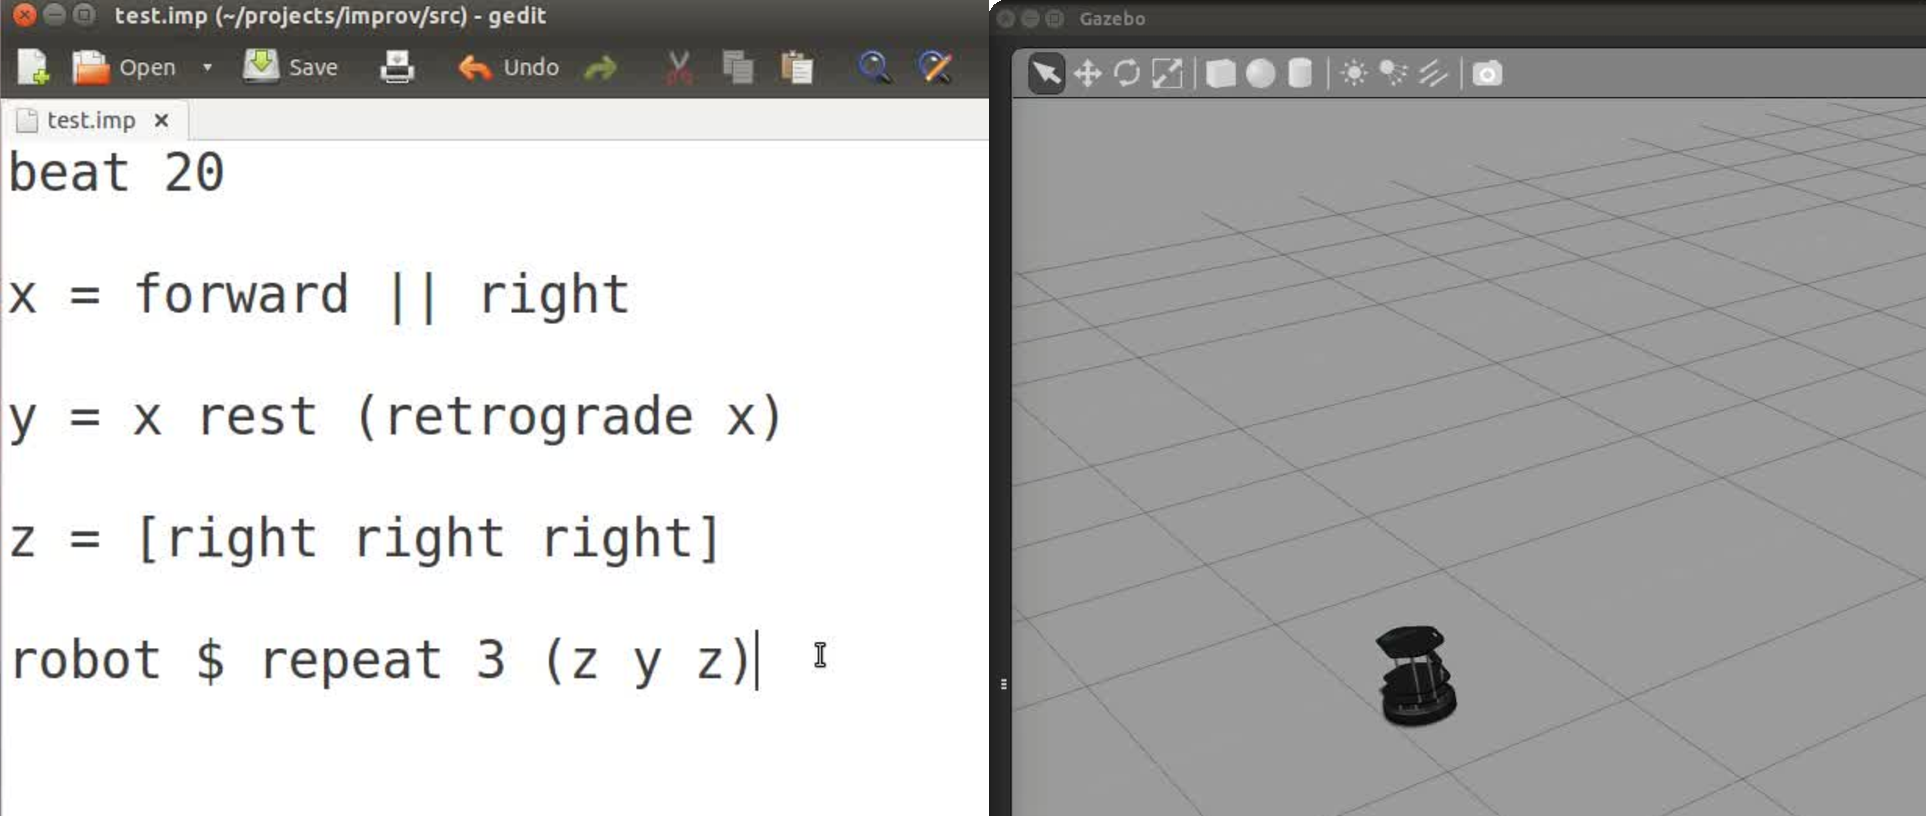
\includegraphics[width=\linewidth]{improv_gedit_gazebo_zoom.pdf}
%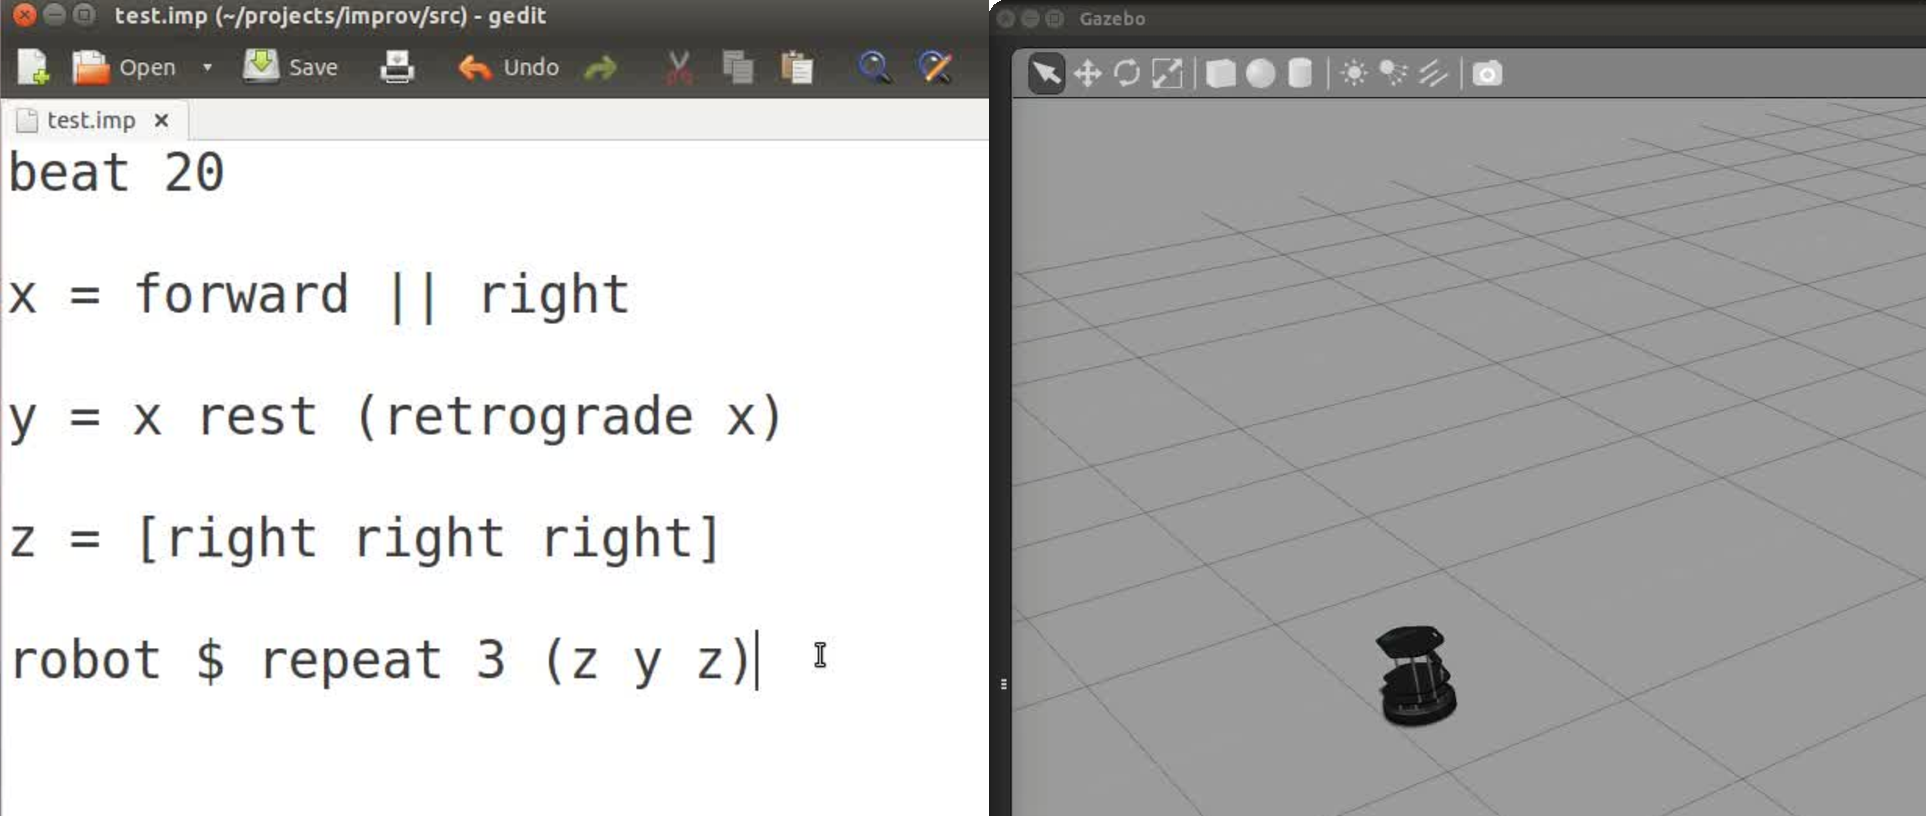
\includegraphics[width=\linewidth,trim={2.5cm 10cm 10cm
%1cm},clip]{improv_gedit_gazebo_zoom.png}
%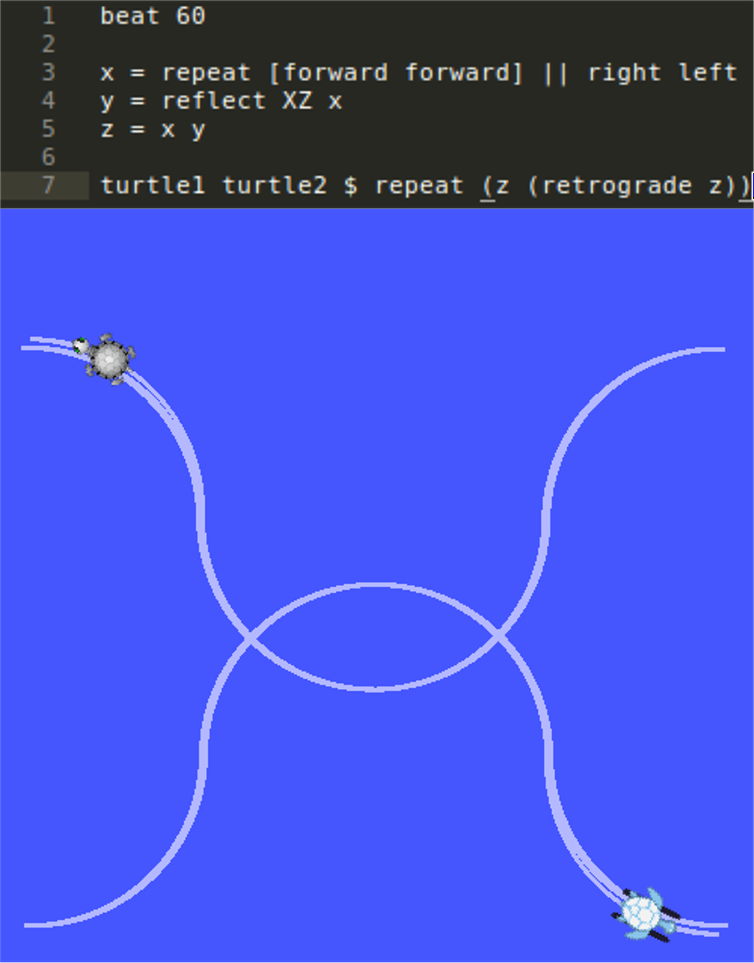
\includegraphics[width=0.7\linewidth]{termturtle.png}
\end{center}

\vspace{0.5em}
}


%----------------------------------------------------------------------------------------
%	APPROACH
%----------------------------------------------------------------------------------------

\headerbox{Design
Principles}{name=approach,column=0,span=1,below=interface,bottomaligned=approach}{
\raggedright
\begin{itemize}\compresslist
\item minimize ``representational distance" between intended movement and code 
\item rapid movement prototyping
\item workspace with few attentional switches
\end{itemize}


}


%----------------------------------------------------------------------------------------
%	Problem Formulation
%----------------------------------------------------------------------------------------


\headerbox{Information Flow}{name=info,column=1,row=0,span=1}{

\begin{center}
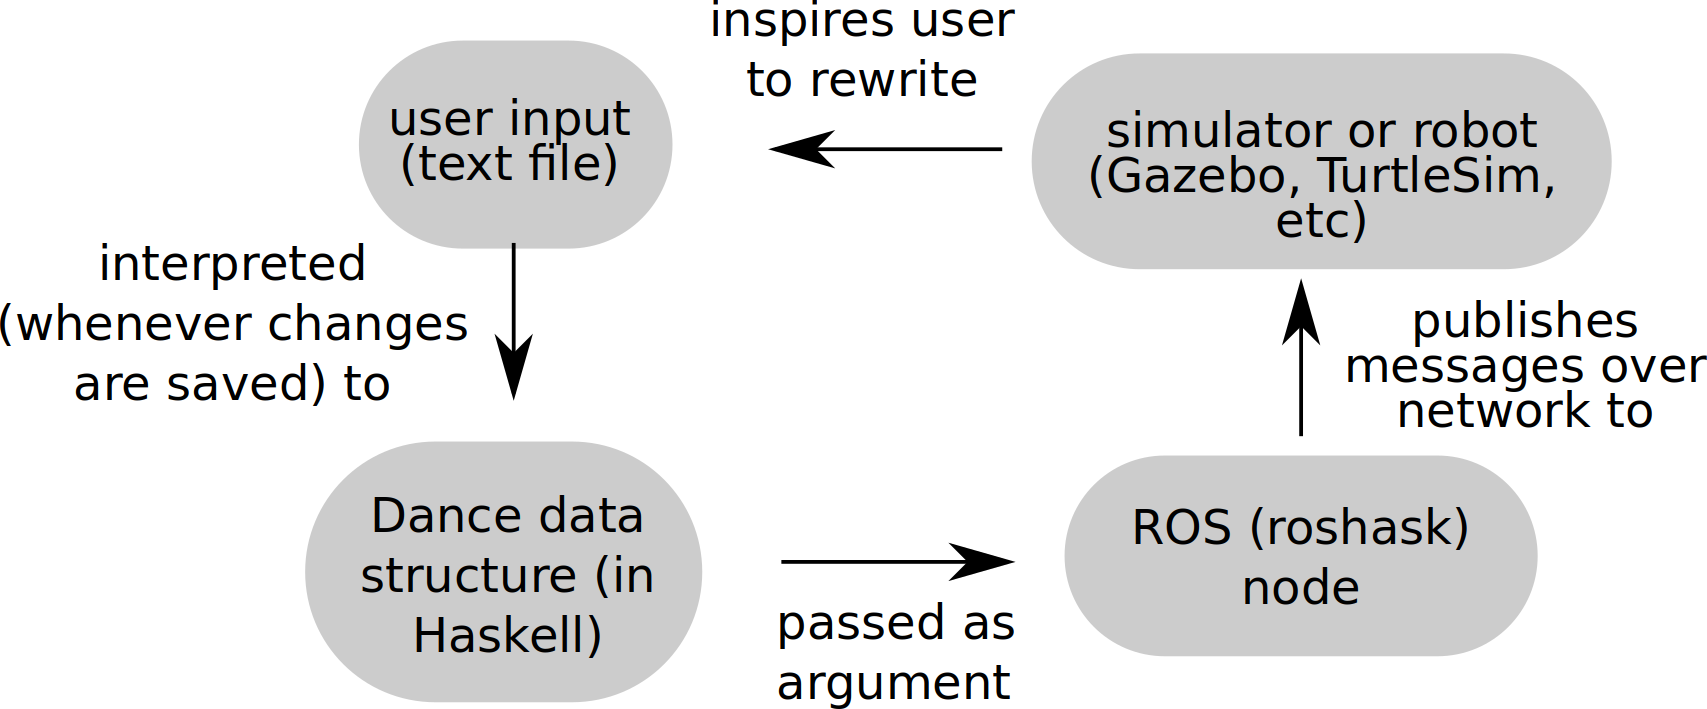
\includegraphics[width=\linewidth]{flowchart.pdf}
\end{center}

}


%----------------------------------------------------------------------------------------
%	LIMIT CYCLES IN CONVEX POLYGONS
%----------------------------------------------------------------------------------------

\headerbox{Expressive Building Blocks}{name=convex,column=1,bottomaligned=approach,below=info,span=1}{

\begin{center}
\textbf{Combining Movements}
\end{center}

\emph{move forward for one beat, turn right for one beat, move forward for one beat} \\
\texttt{forward right forward} \\

\vspace{-0.5em}

\emph{move forward, right, and forward, all in one beat} \\
\texttt{[forward right forward]} \\

\vspace{-0.5em}

\emph{move in a curve, forward and right} \\
\texttt{forward \textbar{}\textbar{} right} \\

\vspace{-1em}

\begin{center}
\textbf{Transforming Movements}
\end{center}

\emph{move forward four times} \\
\texttt{repeat 4 forward} \\

\vspace{-0.5em}

\emph{do movement \texttt{x}, reflected across saggital plane} \\
\texttt{reflect YZ x} \\

\vspace{-0.5em}

\emph{reverse "forward right left"} \\
\texttt{reverse (forward right left)} \\

\vspace{-0.5em}

\emph{retrograde "forward right left"} \\
\texttt{retrograde (forward right left)} 
}


%----------------------------------------------------------------------------------------
%	RESULTS 2
%----------------------------------------------------------------------------------------
%\headerbox{Ongoing Work: Coverage
%Properties}{name=chaos,column=2,span=1,below=nonconvex}{ 
%
%\begin{multicols}{2}
%
%\begin{center}
%\includegraphics[width=0.7\linewidth]{pent_chaos.pdf}
%\end{center}
%
%\raggedright
%\begin{itemize}\compresslist
%\item Are trajectories ergodic?
%\item Density of contact with boundary over time?
%\end{itemize}
%
%\end{multicols}
%
%}

%----------------------------------------------------------------------------------------
%	Question
%----------------------------------------------------------------------------------------

\headerbox{Comparing Representations}{name=question,row=0,column=2,span=1}{

%\begin{multicols}{2}
\vspace{1em}
{\large
\begin{center}
\textbf{\Large ROS Program in Python}
\end{center}
\begin{tabular}{l}
\texttt{if \_\_name$\_\_ ==$ '\_\_main\_\_':} \\ 
\MyIndent \texttt{pub = rospy.Publisher(} \\
\MyIndent \MyIndent \texttt{'turtle1/cmd\_vel',Twist)} \\ 
\MyIndent \texttt{rospy.init\_node('publisher\_node')} \\ 
\MyIndent \texttt{loop\_rate = rospy.Rate(5)} \\ 
\MyIndent \texttt{while not rospy.is\_shutdown():} \\ 
\MyIndent \MyIndent        \texttt{vel=Twist()} \\
\MyIndent \MyIndent        \texttt{vel.linear.x = 1.0} \\
\MyIndent \MyIndent        \texttt{vel.angular.z = 1.0} \\
\MyIndent \MyIndent        \texttt{pub.publish(vel)} \\
\MyIndent \MyIndent        \texttt{loop\_rate.sleep()}
}
\end{tabular}

\vspace{1em}

\begin{center}
\textbf{\Large Equivalent Program in Improv}
\end{center}

\texttt{turtle1 \$ forward || left}

\vspace{1em}
%\end{multicols}
%
%\hspace{0em}

}


%----------------------------------------------------------------------------------------
%	FORMAL METHODS
%----------------------------------------------------------------------------------------

\headerbox{Future Work}{name=fm,column=2,span=1,below=question}{
\raggedright
\begin{itemize}\compresslist
\item More articulated robots: how to represent in platform-invariant way?
\item Robot-robot and robot-environment interaction: \texttt{approach},
\texttt{landmarks}, conditional expressions
\item User studies:
    \begin{itemize}\compresslist
    \item How does percieved usability depend on programming experience?
    \item Does the live interface enable creativity? What is the effect of
          delay?
    \end{itemize}
\end{itemize}

}




%----------------------------------------------------------------------------------------
%	CONCLUSIONS
%----------------------------------------------------------------------------------------



%----------------------------------------------------------------------------------------
%----------------------------------------------------------------------------------------
%	ACKNOWLEDGMENTS
%----------------------------------------------------------------------------------------

\headerbox{Acknowledgments}{name=acknowledgments,column=2,span=1,bottomaligned=convex,
below=fm}{
\footnotesize{
\textbf{Funding}: 
This work is partially funded by NSF grant \#1328018 and DARPA grant \#D16AP00001.
%\vspace{-3.5em}
}
%\printbibliography[heading=none]


}
%----------------------------------------------------------------------------------------
%	REFERENCES
%----------------------------------------------------------------------------------------

%\headerbox{References}{name=references,column=1,above=bottom}{
%
%\tiny{
%
%
%1. Woese, C., et al. PNAS, 4576–4579 (1990).\\
%2. Zomer, A., et al. PLoS ONE 7, e43012 (2012).\\
%3. Solaimanpour, S., et al. PLOS ONE 10, e0126070 (2015).\\
%4. Makarova, K., , et al. Life 5, 818–840 (2015).
%
%
%}}
%
%----------------------------------------------------------------------------------------
%	FUTURE RESEARCH
%----------------------------------------------------------------------------------------
%
%\headerbox{Future Research}{name=futureresearch,column=1,span=2,aligned=references,above=bottom}{ % This block is as tall as the references block
%
%\begin{multicols}{2}
%Integer sed lectus vel mauris euismod suscipit. Praesent a est a est ultricies pellentesque. Donec tincidunt, nunc in feugiat varius, lectus lectus auctor lorem, egestas molestie risus erat ut nibh.
%
%Maecenas viverra ligula a risus blandit vel tincidunt est adipiscing. Suspendisse mollis iaculis sem, in \emph{imperdiet} orci porta vitae. Quisque id dui sed ante sollicitudin sagittis.
%\end{multicols}
%}
%




\end{poster}

\end{document}
